% VUT FIT MITAI
% MSZ 2021/2022
% Author: Vladimir Dusek
% Login: xdusek27

%%%%%%%%%%%%%%%%%%%%%%%%%%%%%%%%%%%%%%%%%%%%%%%%%%%%%%%%%%%%%%%%%%%%%%%%%%%%%%%%

% Path to figures
\graphicspath{{avs/pametova_konzistence/figures}}

%%%%%%%%%%%%%%%%%%%%%%%%%%%%%%%%%%%%%%%%%%%%%%%%%%%%%%%%%%%%%%%%%%%%%%%%%%%%%%%%

\chapter{AVS~--~Paměťová konzistence a předbíhání operací čtení a zápisu, podpora virtuálního adresového prostoru.}

%%%%%%%%%%%%%%%%%%%%%%%%%%%%%%%%%%%%%%%%%%%%%%%%%%%%%%%%%%%%%%%%%%%%%%%%%%%%%%%%

\section{Zdroje}

\begin{compactitem}
    \item \path{AVS-03.pdf}
    \item \path{AVS-04.pdf}
    \item \path{AVS_2019-10-07.mp4}
    \item \path{AVS_2019-10-14.mp4}
\end{compactitem}

%%%%%%%%%%%%%%%%%%%%%%%%%%%%%%%%%%%%%%%%%%%%%%%%%%%%%%%%%%%%%%%%%%%%%%%%%%%%%%%%

\section{Paměti cache (rychlé vyrovnávací paměti)}

\begin{compactitem}
    \item K čemu je? \begin{compactitem}
        \item Snížení objemu komunikace s hlavní pamětí.
        \item Snížení průměrné doby přístupu.
    \end{compactitem}

    \item Jelikož malé paměti jsou rychlejší a dražší, velké paměti pomalejší a levnější, je optimální paměťový systém hierarchický -- Úrovně cache: L1C, L2C, L3C.

    \item Datová cache a instrukční cache.

    \item Metriky: \begin{compactitem}
        \item Cache miss -- data v cache nejsou.
        $$ \text{miss rate} = \frac{\text{cache miss}}{\text{celkový počet přístupů}} $$

        \item Cache hit -- data v cache jsou (cache hit / celkový počet = hit rate).
        $$ \text{hit rate} = \frac{\text{cache hit}}{\text{celkový počet přístupů}} $$
    \end{compactitem}

    \item Velikost jednoho bloku cache je typicky 64\,B (celková velikost je např. 16\,KB). \begin{compactitem}
        \item Z paměti do cache vždy bereme celý blok.
    \end{compactitem}

    \item Platí princip časové a prostorové lokality.

    \item Vzhledem ke klesající velikosti paměti se vzrůstající úrovní hierarchie musí existovat mapování: \begin{compactitem}
        \item přímé mapování;
        \item plně asociativní;
        \item skupinově asociativní (nejpoužívanější).
    \end{compactitem}

    \begin{figure}[H]
        \centering
        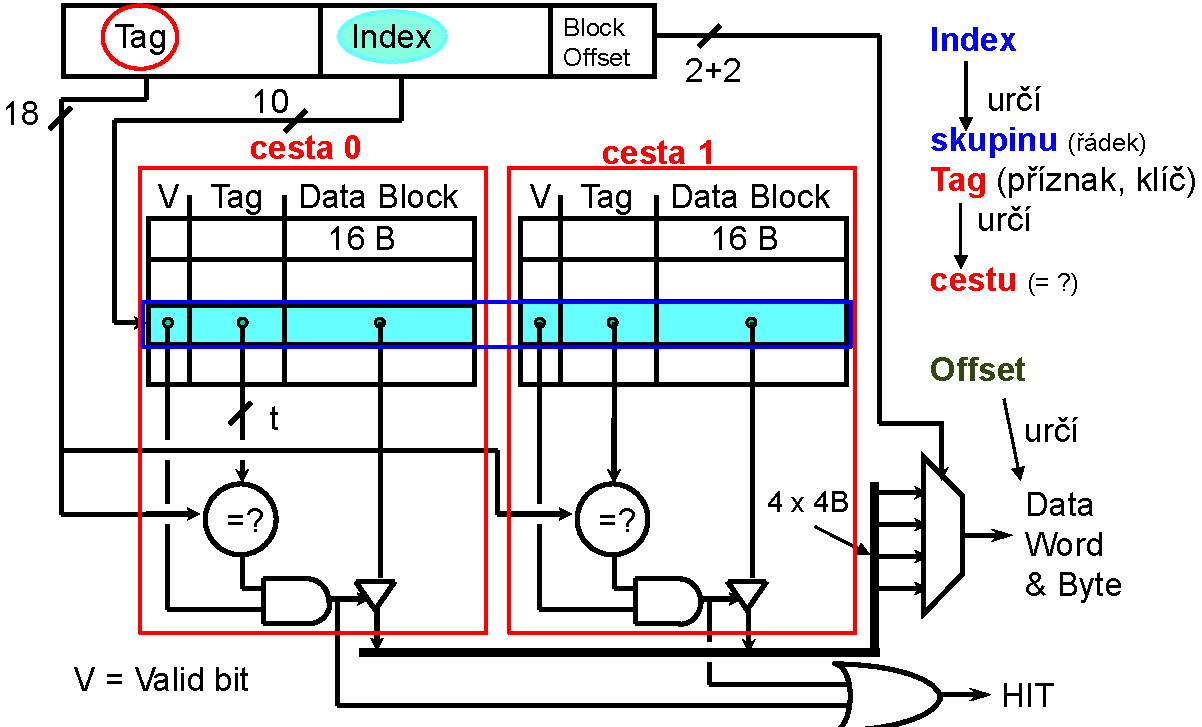
\includegraphics[width=0.9\linewidth]{skupinove_asociativni_cache.pdf}
        \caption{Skupinově asociativní cache.}
    \end{figure}

    \item Strategie výběru bloku pro přemístění z cache do paměti: \begin{compactitem}
        \item LRU (\textit{last recently used}) -- blok nejdéle nepoužitý, zaznamenává se počet přístupů;
        \item FIFO -- nejstarší blok;
        \item náhodný.
    \end{compactitem}

    \begin{figure}[H]
        \centering
        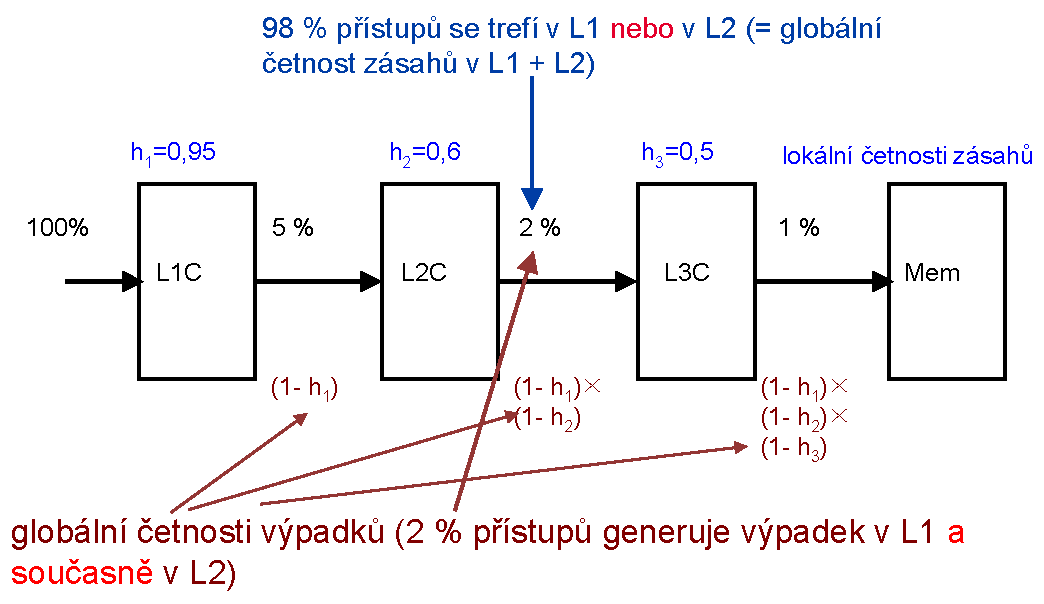
\includegraphics[width=1\linewidth]{lokalni_a_globalni_cetnost_vypadku.pdf}
        \caption{Lokální a globální četnost výpadků a zásahů.}
    \end{figure}
\end{compactitem}

%%%%%%%%%%%%%%%%%%%%%%%%%%%%%%%%%%%%%%%%%%%%%%%%%%%%%%%%%%%%%%%%%%%%%%%%%%%%%%%%

\section{Podpora virtuální paměti}

\begin{compactitem}
    \item Každý proces \uv{vidí} paměť po svým (od \path{000...} až po \path{fff...}). -- Procesy jsou od sebe \uv{odstíněny}.

    \item Pamět dělíme na tzv. stránky (\textit{page}). \begin{compactitem}
        \item Velikost stránky je typicky 4\,KB (lze změnit).
        \item Mapování mezi fyzickým a virtuálním adresovým prostorem probíhá po stránkách.
    \end{compactitem}

    \item Máme dva adresované prostory: \begin{compactitem}
        \item Virtuální adresa (VA) = adresa virtuální stránky (VPN, \textit{virtual page number}) + číslo bloku na stránce (\textit{page offset}).
        \item Fyzická adresa (PA) = (PPN, \textit{physical page number}) + číslo bloku na stránce (\textit{page offset}).
    \end{compactitem}

    \item Page offset -- číslo bloku na stránce.
    \item Block offset -- které slovo/byte.

    \item MMU (\textit{memory management unit}) -- Jednotka správy paměti v procesoru, která provádí překlad adres.

    \item Překlad: \begin{compactitem}
        \item Překládání na úrovni stránek.
        \item Více-úrovňová tabulka stránek.
    \end{compactitem}

    \begin{figure}[H]
        \centering
        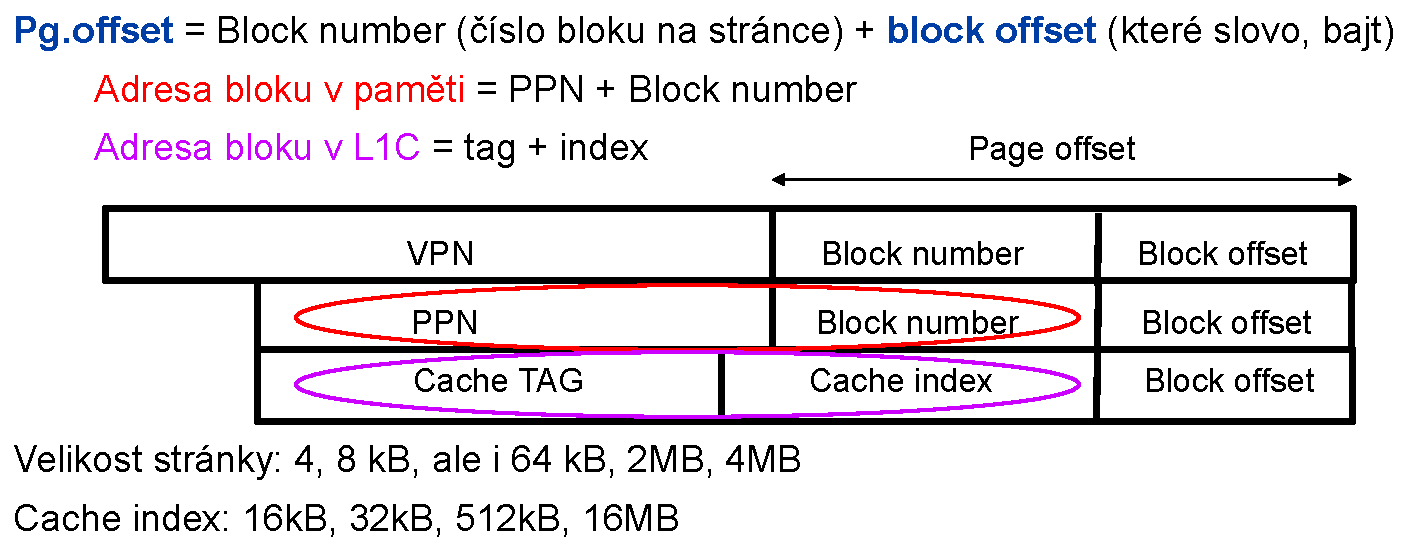
\includegraphics[width=0.9\linewidth]{podpora_virtualni_pameti.pdf}
        \caption{Podpora virtuální paměti.}
    \end{figure}
\end{compactitem}

\subsection{Lineární tabulka stránek (PT, \textit{page table})}

\begin{compactitem}
    \item Byla by příliš velká, takhle to udělat nejde.

    \begin{figure}[H]
        \centering
        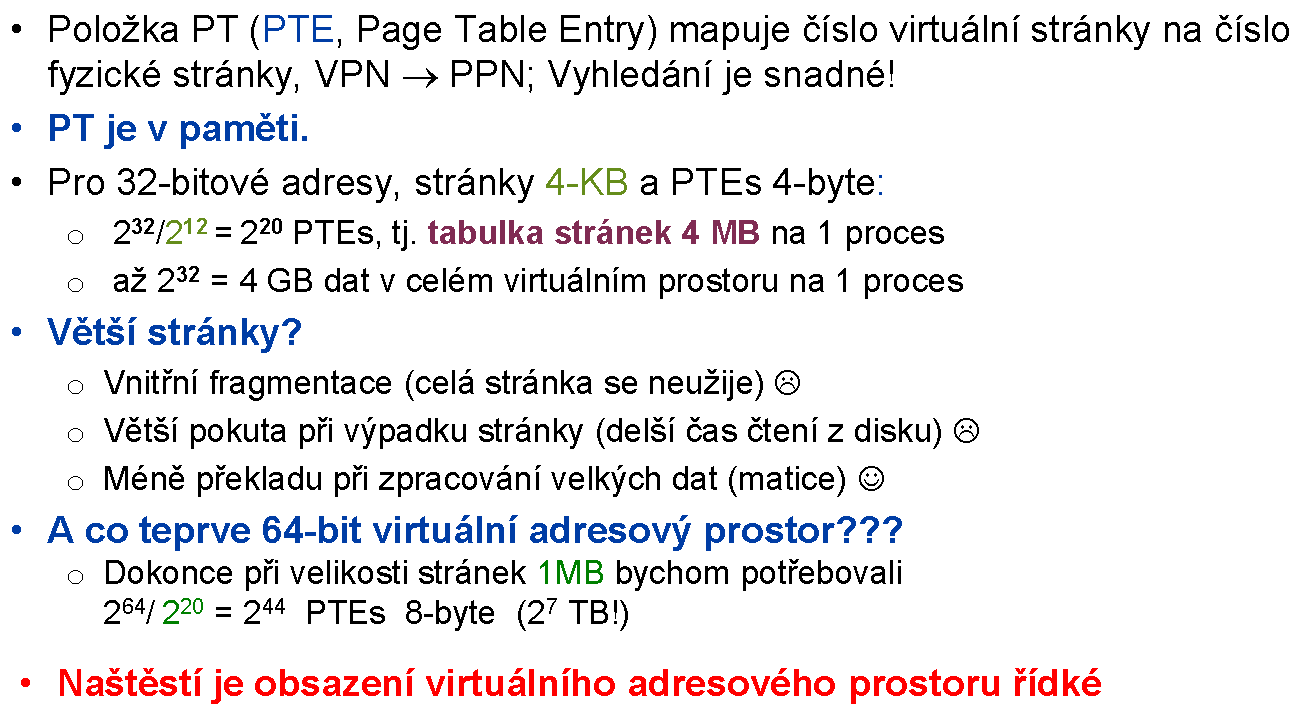
\includegraphics[width=1\linewidth]{linearni_tabulka_stranek.pdf}
        \caption{Velikost lineární tabulky stránek.}
    \end{figure}
\end{compactitem}

\subsection{Více-úrovňová tabulka stránek}

\begin{compactitem}
    \item Hierarchická struktura (n-ární strom).
    \item Výhody: \begin{compactitem}
        \item ušetříme paměť;
        \item ušetříme rychlost vyhledávání.
    \end{compactitem}

    \item Nevýhoda: \begin{compactitem}
        \item Tabulky stránek jsou uloženy v paměti, přístup do paměti je drahý. Řešíme pomocí hardwaru, tzv. TLB (\textit{translation lookaside buffer}).
    \end{compactitem}

    \begin{figure}[H]
        \centering
        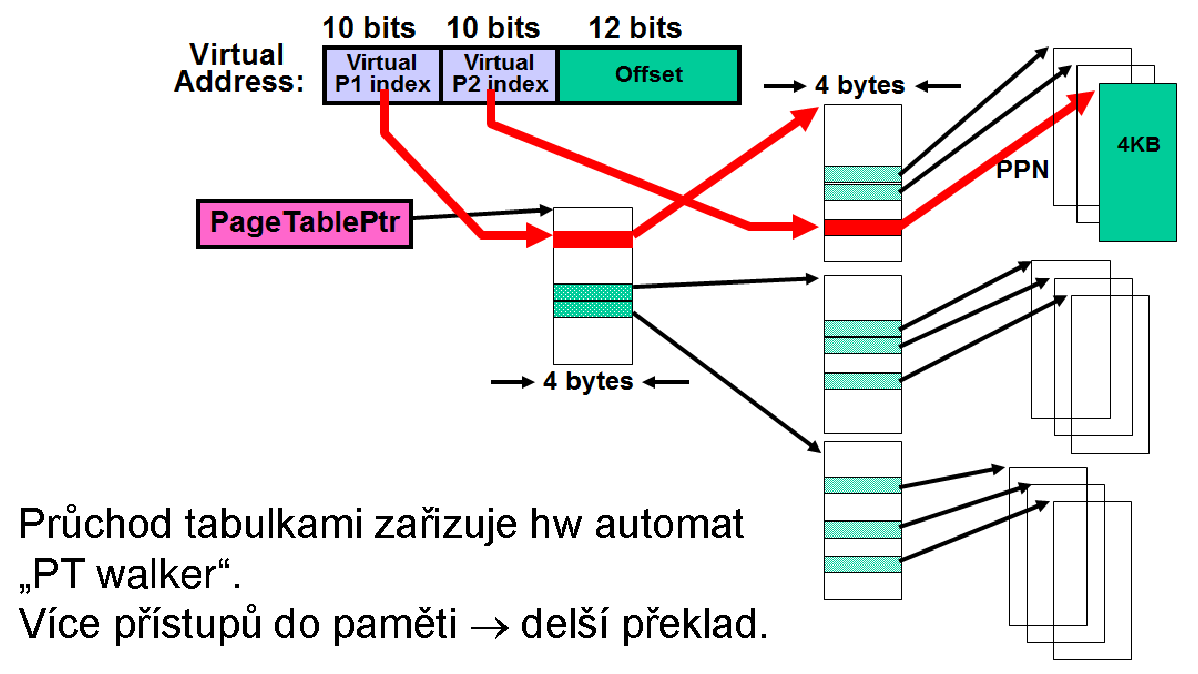
\includegraphics[width=1\linewidth]{viceurovnova_tabulka_stranek.pdf}
        \caption{Více-úrovňová tabulka stránek.}
    \end{figure}

    \begin{figure}[H]
        \centering
        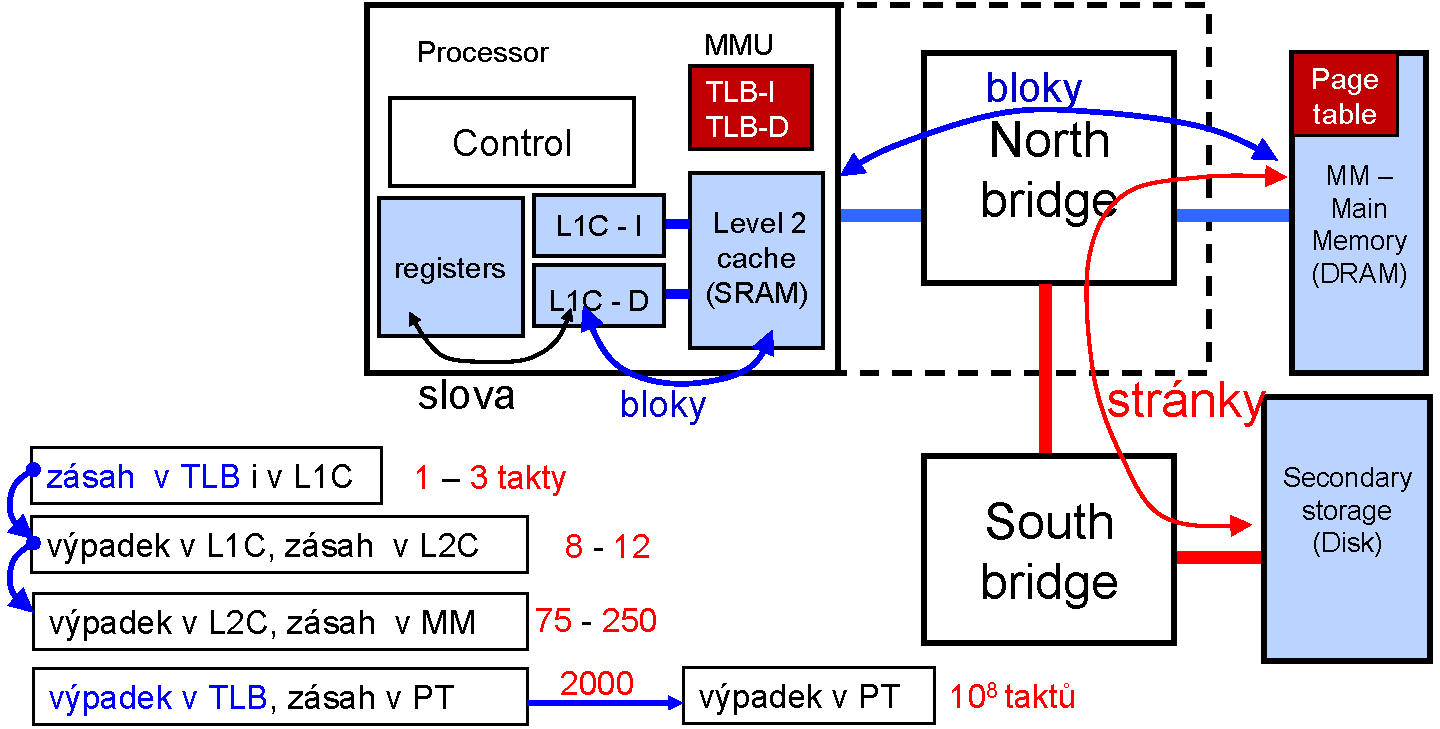
\includegraphics[width=1\linewidth]{pameti_cache_v_systemu_virtualni_pameti.pdf}
        \caption{Paměti cache v systému virtuální paměti.}
    \end{figure}

    \begin{figure}[H]
        \centering
        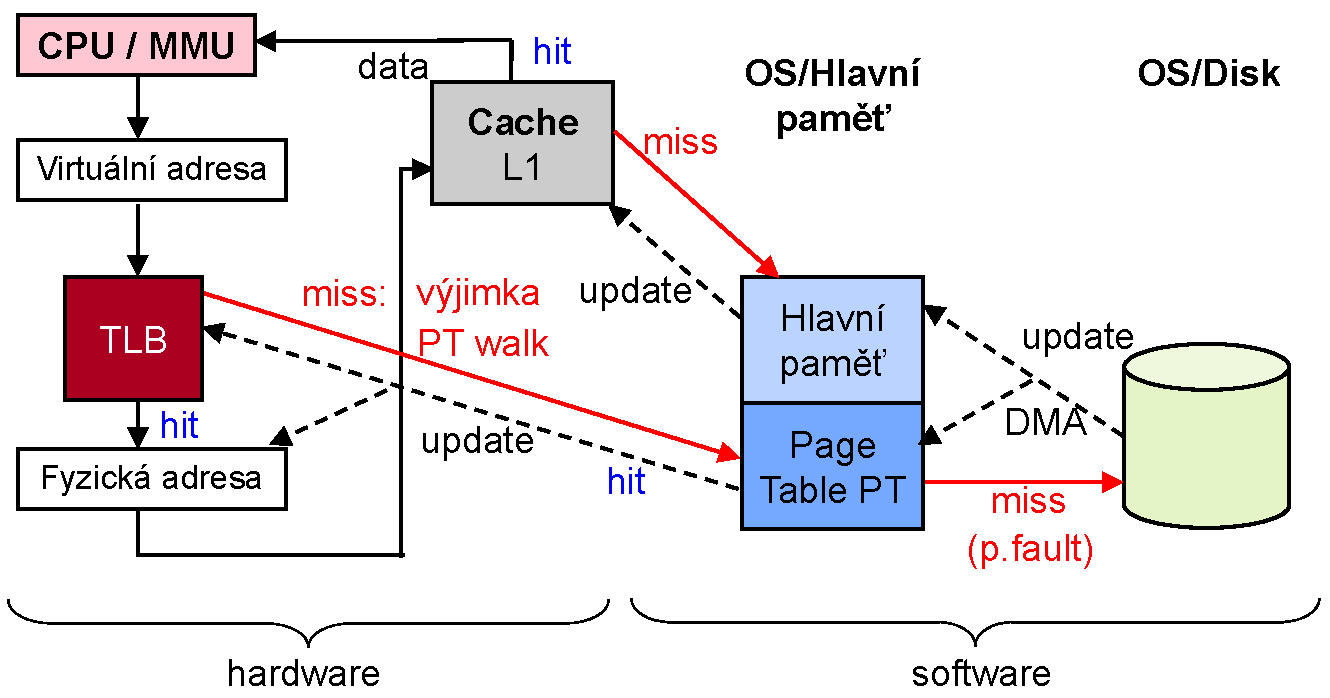
\includegraphics[width=1\linewidth]{schema_pristupu_do_pameti.pdf}
        \caption{Schéma přístupu do paměti s L1C.}
    \end{figure}
\end{compactitem}

\subsection{TLB (\textit{translation lookaside buffer})}

\begin{compactitem}
    \item Cache pro překlad stránek, která je umístěna na procesoru a obsahuje sadu aktuálně používaných dvojic (VPN, PPN).

    \item Plně asociativní.

    \begin{figure}[H]
        \centering
        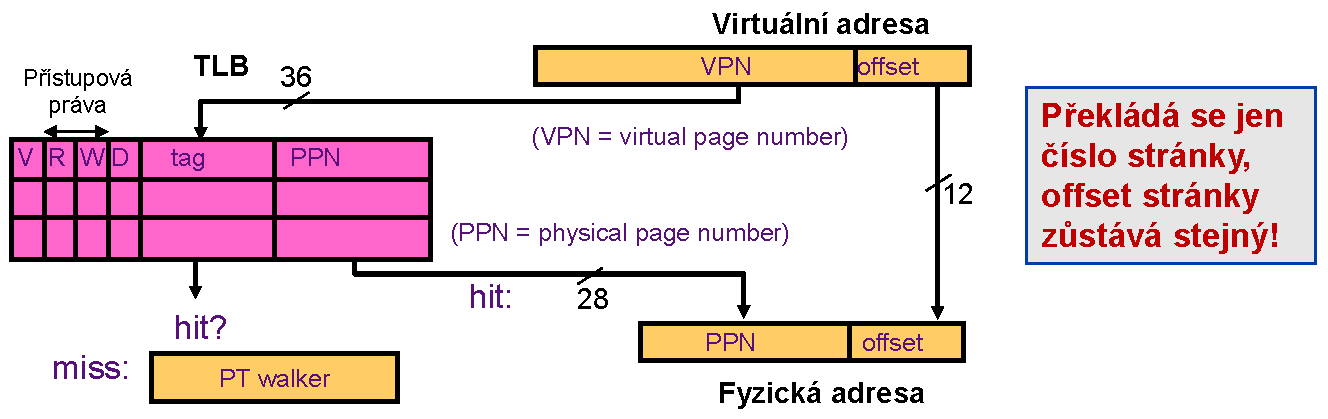
\includegraphics[width=1\linewidth]{tlb.pdf}
        \caption{TLB.}
    \end{figure}
\end{compactitem}

\subsection{Virtuální paměť a cache}

\begin{compactitem}
    \item Spolupráce s CPU a L1C vyžaduje co nejrychlejší přístup do cache.

    \item Jak dospět od virtualní adresy k adrese bloku (index, tag) v L1C? \begin{compactitem}
        \item virtuální adresa je k dispozici ihned;
        \item fyzická adresa je k dispozici až po překladu VA;
    \end{compactitem}

    \item Která adresa by se mohla použít pro přístup? Tři možnosti: \begin{compactitem}
        \item P/P cache: fyzický index, fyzický tag
        \item V/V cache: virtutální index, virtutální tag
        \item V/P cache: virtutální index, fyzický tag
        \item P/V cache: fyzický index, virtuální tag -- nepoužívá se, index by se musel získat překladem a čas se neuspoří.
    \end{compactitem}
\end{compactitem}

%%%%%%%%%%%%%%%%%%%%%%%%%%%%%%%%%%%%%%%%%%%%%%%%%%%%%%%%%%%%%%%%%%%%%%%%%%%%%%%%

\section{Optimalizace toku dat přes paměť (předbíhání)}

\begin{compactitem}
    \item Stupně L/S jednotky: \begin{compactitem}
        \item generování (výpočet) adresy;
        \item překlad z virtuální na fyzickou adresu;
        \item přístup do cache (adresace).
    \end{compactitem}

    \item Mezi instrukcemi Load a Store se stejnou adresou existují datové závislosti, podobně jako u registrů. \begin{compactitem}
        \item RAW, WAR, WAW.
        \item Není je možné odhalit dříve než jsou spočteny adresy paměťových operandů.
        \item Závislosti musí být respektovány, aby se zachovala sémantika programu, jinak vzniká paměťová nekonzistence.
    \end{compactitem}

    \item Instrukce Load a Store je možné vykonávat podle pořadí v programu, což může být pomalé. A nebo za jistách okolností můžou být vykonávány mimo pořadí: \begin{compactitem}
        \item RPR (read can pass read);
        \item RPW (read can pass write);
        \item WPR (write can pass read);
        \item WPW (write can pass write) -- Když jdou na jiné adresy.
    \end{compactitem}
\end{compactitem}

\subsection{Read can pass write (RPW)}

\begin{compactitem}
    \item Tzv. bypassing (přeskočení dopředu) a forwarding (zkratka).
    \begin{figure}[H]
        \centering
        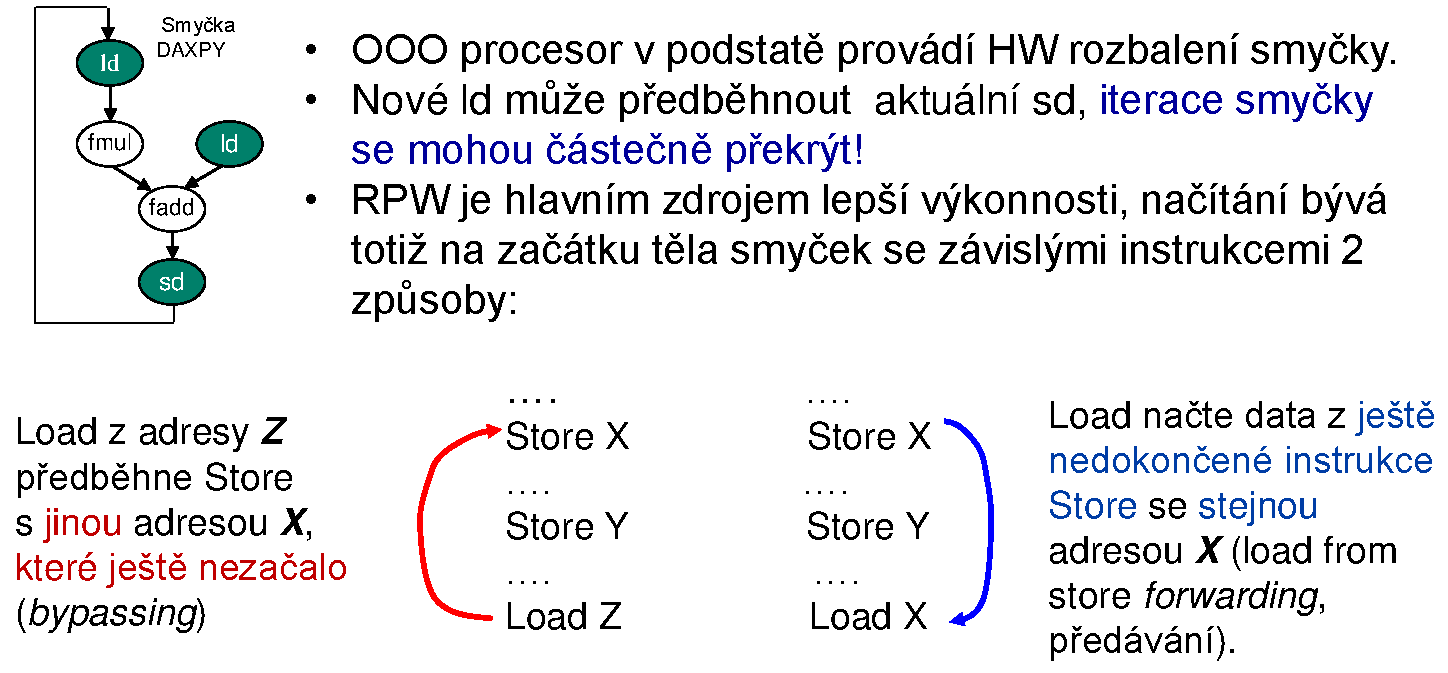
\includegraphics[width=1\linewidth]{rpw.pdf}
        \caption{RPW, příklad smyčka DAXPY.}
    \end{figure}

    \item Potřebujeme techniku dynamického rozlišování adres: adresa(R) $\not=$ adresa(W)?
    \item neshoda -- není konflikt RAW, R nečeká na W a předbíhá;
    \item shoda -- R načte data do dst reg z čekajícího nedokončeného zápisu (store bufferu);
    \item neví - čeká nebo spekuluje (předpokládá, že se liší).
\end{compactitem}

\subsection{Store buffer}

\begin{compactitem}
    \item Položka je ve store bufferu alokována v době dekódování (DI). Pokud je store buffer plný, musí se čekat.
    \item Adresy instrukcí Store jsou ve bufferu v programovém pořadí.
    \item Nové adresy Load se kontrolují s čekajícími adresami Store na shodu/neshodu.
    \item Když je instrukce Store na čele ROB i store buferu, dojde k propuštění Store, tj. k zápisu do Dcache. Položka přejde do stavu Available.

    \begin{figure}[H]
        \centering
        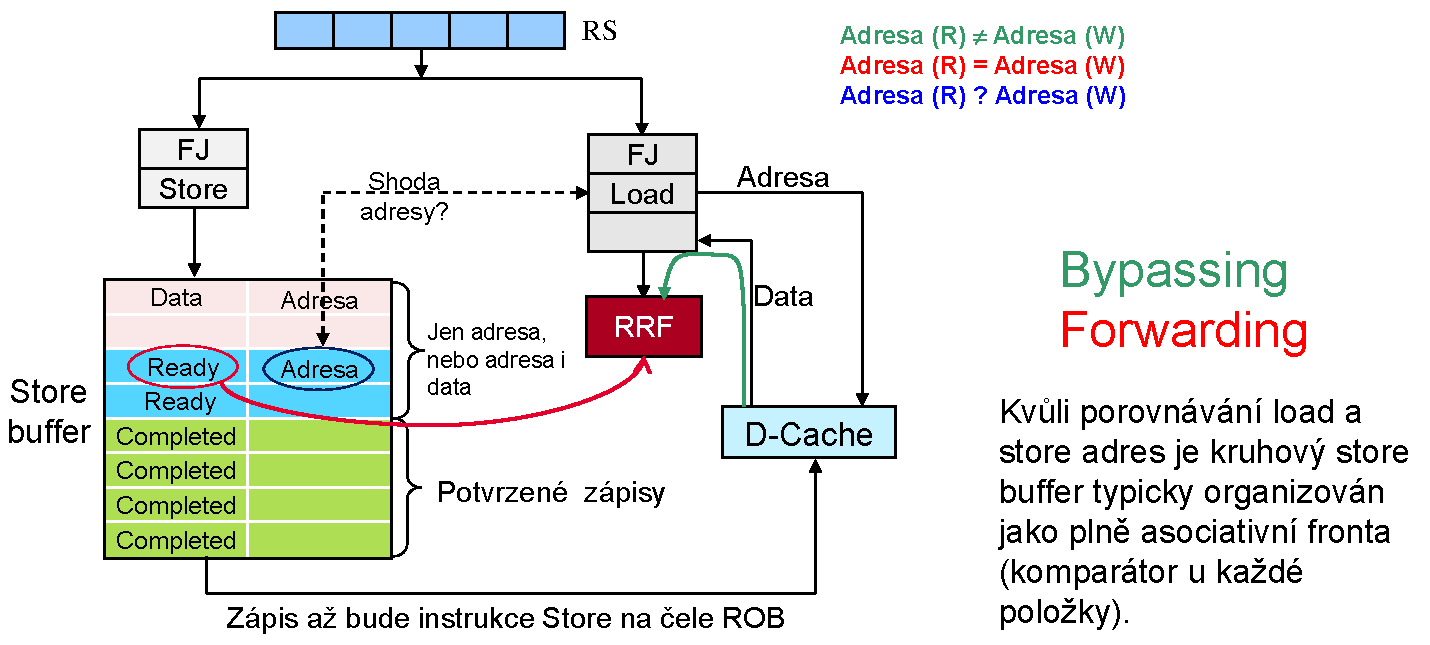
\includegraphics[width=1\linewidth]{store_buffer.pdf}
        \caption{Organizace jednotky L/S podporující RPW.}
    \end{figure}
\end{compactitem}

\subsection{Load buffer}

\begin{compactitem}
    \item Tabulka pro spekulativní načítání.

    \item Pokud některé adresy Store nejsou známy, je třeba spekulovat, že se budou lišit od adresy Load.

    \item Pro ověření spekulace jsou adresy doběhlých spekulativních načítání uloženy do nového L-bufferu.

    \item Každá potvrzená instrukce Store pak musí ověřit, že nemá adresu shodnou s nějakou položkou L-bufferu, tj. s nějakým spekulativním čtením, které Store předběhlo. \begin{compactitem}
        \item Při shodě je potřeba postiženou instrukci Load a další za ní následující instrukce zrušit a opakovat.
        \item Pokud k žádné shodě nedošlo až do dokončení Store, je proveden přepis Load dat z RRF do ARF.
    \end{compactitem}

    \begin{figure}[H]
        \centering
        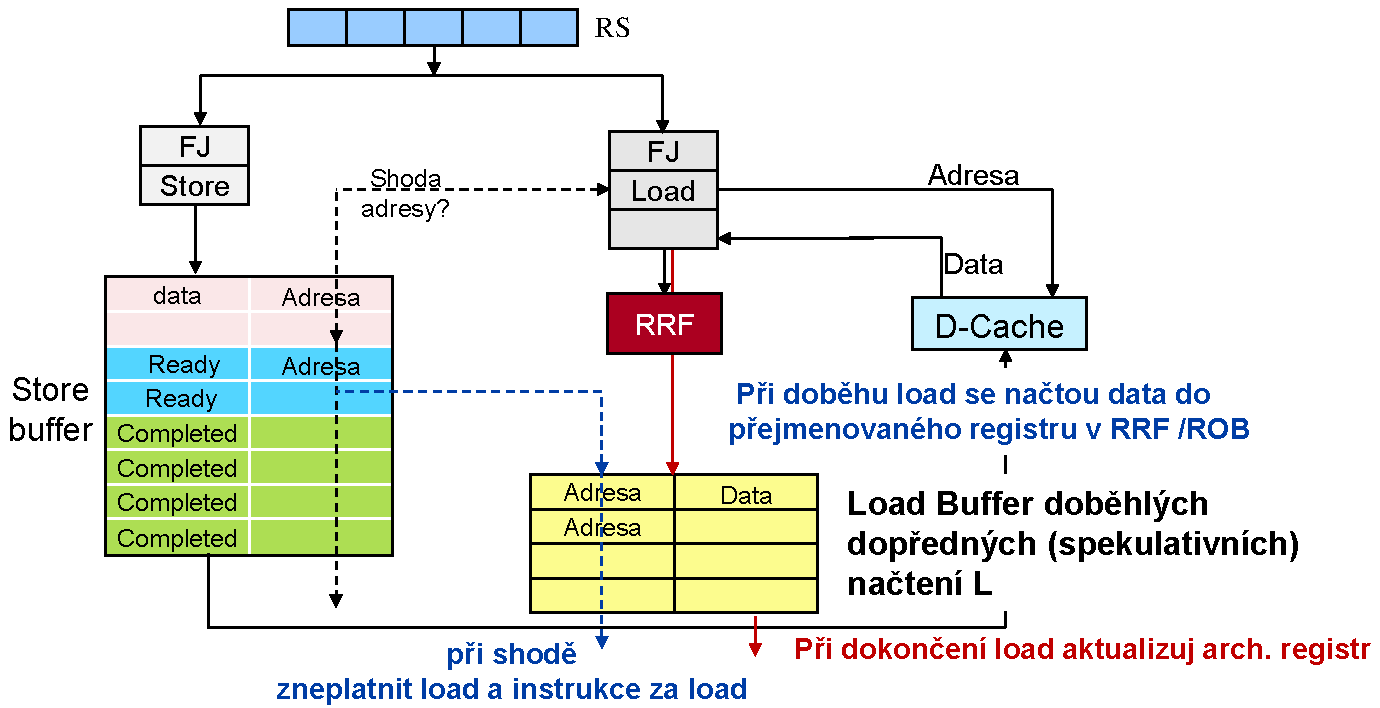
\includegraphics[width=1\linewidth]{load_buffer.pdf}
        \caption{Out-of-order Load / Store jednotka.}
    \end{figure}
\end{compactitem}

\subsection{Relaxovaná paměťová konzistence}

\begin{compactitem}
    \item Sekvenční konsistence, která zachovává pořadí přístupů do paměti, není v současnosti zajímavá. Je totiž překážkou modernímu hardware a optimalizujícím kompilátorům.

    \item Předbíhání RPW je jen jedna možnost uvolnění pořadí přístupů do paměti, i když pro výkonnost nejvýznamnější.

    \item Existuje však řada ještě volnějších modelů se zcela volným pořadím čtení a zápisů.

    \item Moderní procesory vykazují relaxovanou (uvolněnou) paměťovou konsistenci, kdy se čtení a zápisy mohou vzájemně předbíhat, pokud to nemění správnost programu.

    \item Relaxovaná paměťová konzistence: \begin{compactitem}
        \item Lepší výkonnost a jednodušší HW implementace.
        \item Je ponecháno na programátorovi, aby identifikoval a označil spec. instrukcemi (např. paměťovými bariérami) ty instrukce L/S, které musí být uspořádány.
        \item Všechny ostatní instrukce se mohou provádět mimo pořadí.
    \end{compactitem}

    \item Na vyšší úrovni musí programátor použít synchronizační příkazy pro vymezení oblastí předepsaného pořadí L/S: \begin{compactitem}
        \item direktivou flush v OpenM;
        \item proměnnými volatile.
    \end{compactitem}

    \item Nevýhodou relaxovaných modelů je břímě navíc pro programátora, možnost záludných chyb.
\end{compactitem}
